\label{sec:intro}

Many real-world stochastic planning problems involving resources,
time, or spatial configurations naturally use continuous variables in
both their state and action representation.  For example, in a variant
of the
%\InventoryControl problem, a business must must decide how many
%of each item to reorder subject to uncertain demand, inventory holding
%constraints, and quantity-dependent reordering costs.
\MarsRover\ problem~\cite{bresina02}, a rover must navigate within a
continuous environment and carry out assigned scientific discovery
tasks.  In oversubscribed cases where the \MarsRover\ may not be able
to visit all of its assigned landmarks (e.g., to take pictures) within a
given time horizon, it may still be rewarded to some degree for
partial objective fulfillment (e.g, taking pictures within the
vicinity of the assigned landmarks).  

Previous work on \emph{exact} solutions to continuous state \emph{and}
action settings has been quite limited.  There are well-known exact
solutions in the control theory literature for the case of linear
quadratic Gaussian (LQG) control~\cite{lqgc}, i.e., minimizing a quadratic cost
function subject to linear dynamics with Gaussian additive noise in a
partially observable setting.  However, the transition dynamics and
reward (alternately cost) of such problems are not allowed to be
piecewise --- a restriction that prevents us from solving
problems like the aforementioned \MarsRover\ problem.

To be concrete, let us formalize a simple \MarsRover\ problem that
allows us to demonstrate many of the key contributions of the
paper in a compact form:

\begin{example*}[\MarsRover]
\label{ex:knapsack}
A Mars Rover state consists of its continuous position $x$ along a
given route.  In a given time step, the rover may move an arbitrary
continuous distance $d \in [-10,10]$.  The rover receives its greatest
reward for snapping a picture at $x=0$, which quadratically decreases
to zero at the boundaries of the range $x \in [-2,2]$.  The rover will
automatically take a picture when it starts a time step within the
range $x \in [-2,2]$ and it only receives this reward once; we use
boolean variable $b$ to indicate whether the picture has already been
taken.  Formally, using $x'$ and $b'$ to denote the post-action state
and $R$ to denote the reward function, we obtain a simple instance of
a CSA-MDP:\footnote{One will note that this CSA-MDP example is
deterministic for purposes of minimal exposition; the solution in the
paper will generally allow for CSA-MDPs with discrete noise.}
\begin{align} 
P(b'|x) & = 
\begin{cases}
b \lor (x \geq -2 \land x \leq 2): & 1.0\\
\neg b \land (x < -2 \lor x > 2):  & 0.0
\end{cases} \label{eq:mr_discrete_trans} \\
P(x'|x,d) & = \delta \left( x' - \begin{cases}
d \geq -10 \land d \leq 10 : & \hspace{-2mm} x + d \\
d < -10 \lor d > 10 : & \hspace{-2mm} x
\end{cases}
\right) \label{eq:mr_cont_trans} \\
R(x,b) & = \begin{cases}
\neg b \land x \geq -2 \land x \leq 2 : & 4 - x^2 \\
b \lor x < -2 \lor x > 2 : & 0
\end{cases} \label{eq:mr_reward}
\end{align}
\end{example*}
There are two natural questions that we want to ask in CSA-MDP settings
such as this one:
\begin{enumerate}
\item[(a)] What is the optimal value that can be obtained from any state 
over a fixed time horizon?
\item[(b)] What is the corresponding policy one should execute to
achieve this optimal value?
\end{enumerate}

%%%%%%%%%%%%%%%%%%%%%%%%%%%%%%%%%%%%%%%%%%%%%%%%%%%%%%%%%%%%%%%%%%%%%%%%%%
\begin{figure}[t!]
\centering
%\subfigure{
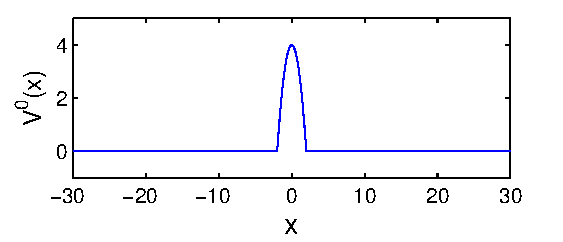
\includegraphics[width=0.4\textwidth]{Figures1/v1_mr.pdf}\\
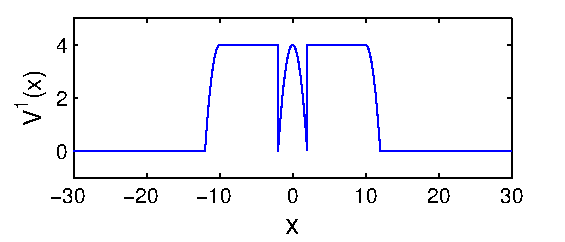
\includegraphics[width=0.4\textwidth]{Figures1/v2_mr.pdf}\\
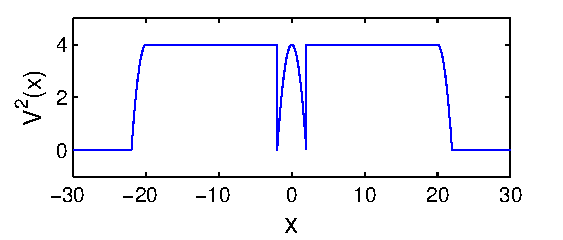
\includegraphics[width=0.4\textwidth]{Figures1/v3_mr.pdf}
\vspace{-2mm}
\caption{\footnotesize Optimal value functions $V^t$ (for $b =
\false$) for time horizons (i.e., decision stages remaining) $t=0$,
$t=1$, and $t=2$ on the \MarsRover\ problem.  For $x \in [-2,2]$, the
rover automatically takes a picture and receives a reward quadratic in
$x$.  For $V^1$, the rover may move up to 10 units in
either direction, reaching the full reward of $4$ up
to $x = \pm 10$ and non-zero reward up to $x = \pm 12$. 
For $V^2$, the rover can move up to 20 units in two time steps,
allowing it to achieve non-zero reward up to $x = \pm 12$.}
\label{fig:opt_graph}
%\vspace{-2mm}
\end{figure}
%%%%%%%%%%%%%%%%%%%%%%%%%%%%%%%%%%%%%%%%%%%%%%%%%%%%%%%%%%%%%%%%%%%%%%%%%%

%%%%%%%%%%%%%%%%%%%%%%%%%%%%%%%%%%%%%%%%%%%%%%%%%%%%%%%%%%%%%%%%%%%%%%%%%%
\begin{figure}[t!]
\centering
%\subfigure{
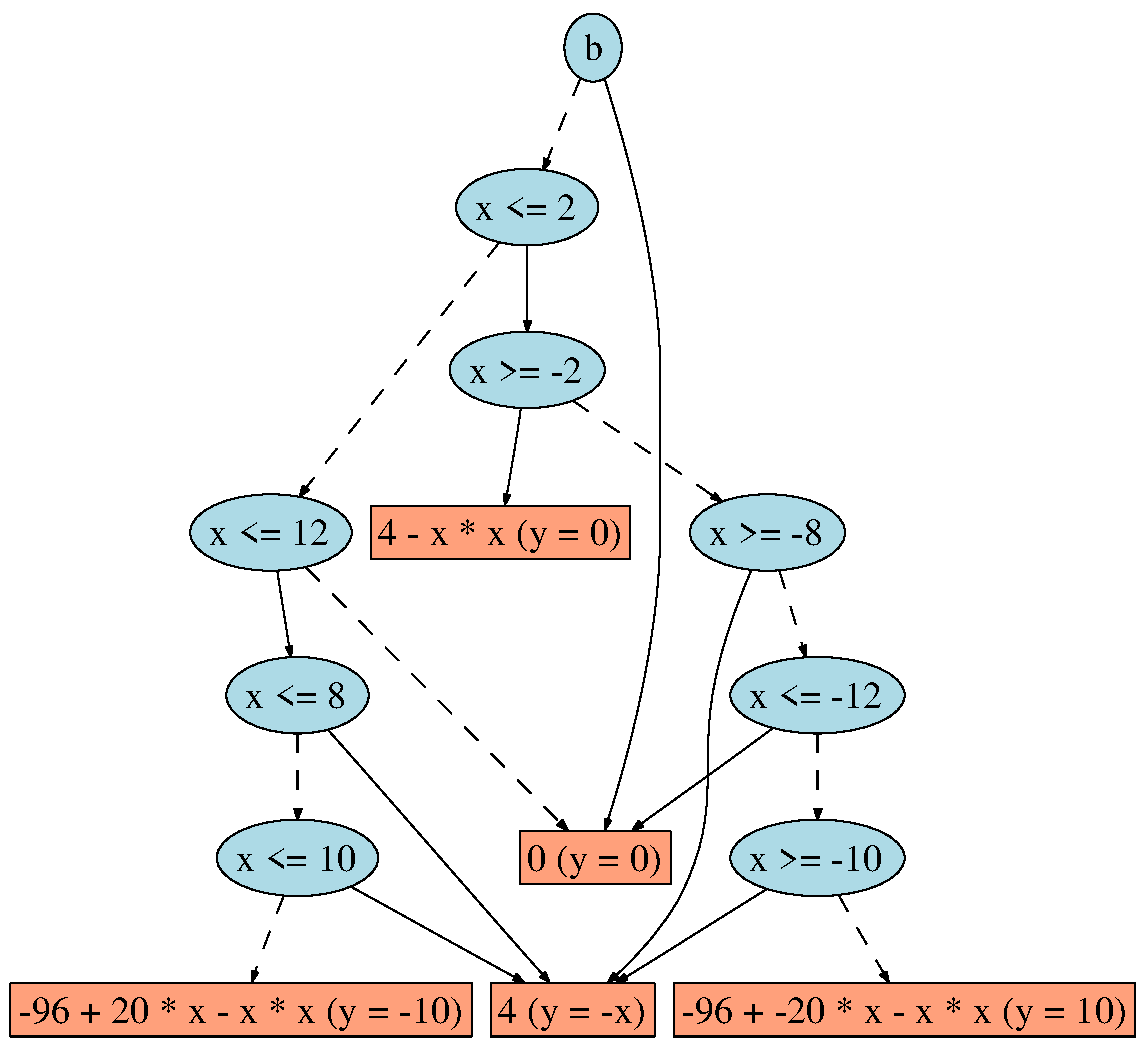
\includegraphics[width=0.5\textwidth]{Figures1/v2_mr_dd.pdf}
%\vspace{-3mm}
\caption{\footnotesize Optimal value function $V^1$ for the
\MarsRover\ problem represented as an extended algebraic decision
diagram (XADD).  Here the solid lines represent the $\true$ branch for
the decision and the dashed lines the $\false$ branch.  To evaluate
$V^1(x)$ for any state $x$, one simply traverses the diagram in a
decision-tree like fashion until a leaf is reached where the
expression provides the value.  The second expression in parentheses
in each leaf provides the optimal action \emph{policy} for $d$ as a
function of the state that allows one to obtain $V^1(x)$.  This
closed-form policy can be derived as a byproduct of symbolic dynamic
programming as we discuss later.}
\label{fig:opt_val_pol}
%\vspace{-3mm}
\end{figure}
%%%%%%%%%%%%%%%%%%%%%%%%%%%%%%%%%%%%%%%%%%%%%%%%%%%%%%%%%%%%%%%%%%%%%%%%%%

To get a sense of the form of the optimal solution to problems such as
the \MarsRover, we present the 0-, 1-, and 2-step time horizon solutions
for this problem in Figure~\ref{fig:opt_graph}; further, in symbolic form,
we display both the 1-step time horizon value function (the 2-step is
too large to display) and corresponding optimal policy in
Figure~\ref{fig:opt_val_pol}.  Here we see that the piecewise 
nature of the transition and reward function lead to
piecewise structure in the value function and policy.  And 
despite their striking simplicity, we are not aware of any exact
solution method to the above \MarsRover\ variant that can produce
such an optimal closed-form result.

To this end, we extend the symbolic dynamic programming (SDP) framework
of~\cite{sanner_uai11} to the case of continuous actions to obtain the
\emph{optimal closed-form} value function and policy for CSA-MDPs with
discrete noise, piecewise linear dynamics, and piecewise quadratic
rewards.  As the fundamental technical contribution of the paper, we
show how the \emph{continuous action maximization} step in the dynamic
programming backup can be evaluated optimally and symbolically and how
it can be efficiently realized in the extended algebraic decision diagram (XADD)
we use to perform all SDP operations.  This
allows us to obtain the \emph{first} algorithm to derive exact closed-form
solutions to this class of CSA-MDPs along with a closed-form
representation of the optimal policy
(cf. Figure~\ref{fig:opt_val_pol}).  
%- extension to XADDs
%- solutions for multivariate actions and quadratic reward
%- automatic derivation of the policy
%- first exact solution to variants of multi-inventory control
%  problem, water reservoir, and quadratic reward problems with
%  piecewise dynamics
We empirically evaluate the time and space required to compute exact
solutions to the \MarsRover\ problem for different time horizons, as
well as \WaterReservoir\ and multivariate action \InventoryControl\
studied in operations research showing the first exact solutions for
these problems can be practically computed for reasonable horizons.
